\documentclass[11pt,a4paper]{article}
\usepackage[T1]{fontenc}\usepackage[utf8]{inputenc}\usepackage{lmodern,amsmath,graphicx,booktabs,array,longtable,microtype,float,placeins,caption,listings,xcolor}
\usepackage[margin=25mm]{geometry}\usepackage[hidelinks]{hyperref}\usepackage{fancyhdr}
\pagestyle{fancy}\fancyhf{}\fancyhead[L]{Square Chimney Heat Transfer}\fancyfoot[C]{\thepage}\setlength{\headheight}{14pt}\setlength{\parindent}{0pt}\setlength{\parskip}{6pt}\setlength{\emergencystretch}{2em}
\captionsetup{font=small,labelfont=bf}\lstset{language=Matlab,basicstyle=\ttfamily\scriptsize,breaklines=true,columns=fullflexible,keepspaces=true,showstringspaces=false,numbers=left,numberstyle=\tiny\color{gray},frame=single,rulecolor=\color{gray!25}}
\begin{document}\begin{titlepage}\centering

\includegraphics[height=22mm]{figures/rId8.png}\hfill
\includegraphics[height=22mm]{figures/rId9.png}\par
\vspace{20mm}{\Large Heat Transfer I\par}\vspace{12mm}{\huge\bfseries Heat Transfer Analysis and Cavity Placement in a Square Chimney\par}\vspace{20mm}
{\Large Pouya Asghari\par}\vfill School of Mechanical Engineering\par College of Engineering, University of Tehran\par Second semester of academic year 1403--1404 (Iranian calendar)\par
\end{titlepage}
\section*{About this translation}
This edition translates the supplied Persian report into English. Source equations, reported data, temperature-array figures, code, and comparison results are retained, with editorial qualifications distinguished from the original numerical statements. The student number is omitted. The original Word drawing overlays are not self-contained raster figures, so the preliminary cavity-location diagrams are reconstructed illustrative grid placements and labeled accordingly.

The MATLAB post-processing mixes Celsius surface temperatures with kelvin ambient temperatures. Consequently, the reported negative heat rates near 18 kW and the resulting optimum are not independently validated physical results. The native files are supplied unchanged; this edition does not silently correct the model or claim a COMSOL rerun.
\begingroup\small\setlength{\parskip}{0pt}\tableofcontents\endgroup\clearpage


\section{Geometry Modeling}

A grid of 10 cm by 10 cm elements is used. The chimney cavity measures 50 cm by 50 cm, and the outside cross section measures 100 cm by 100 cm. With this element size and the intended minimum wall clearance of 10 cm, sixteen grid-aligned cavity positions can be examined. The source initially describes the clearance as greater than 10 cm; its actual grid includes 10 cm clearances.

\begin{figure}[H]\centering

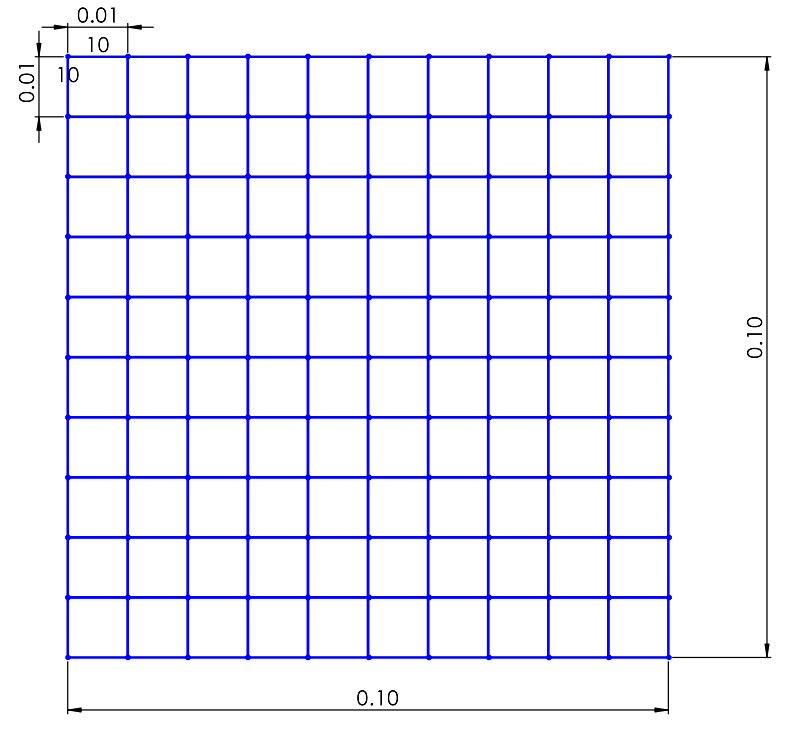
\includegraphics[width=0.94\linewidth,height=0.34\textheight,keepaspectratio]{figures/rId10.png}\par

\caption{Chimney grid with dimensions in meters.}\end{figure}

An initial screening can consider four corner locations and four intermediate locations, followed by refinement in the region with the greatest heat transfer. The diagrams below are reconstructed illustrations of permitted grid placements; the original Word figures combine grid images with drawing overlays.

\begin{figure}[H]\centering

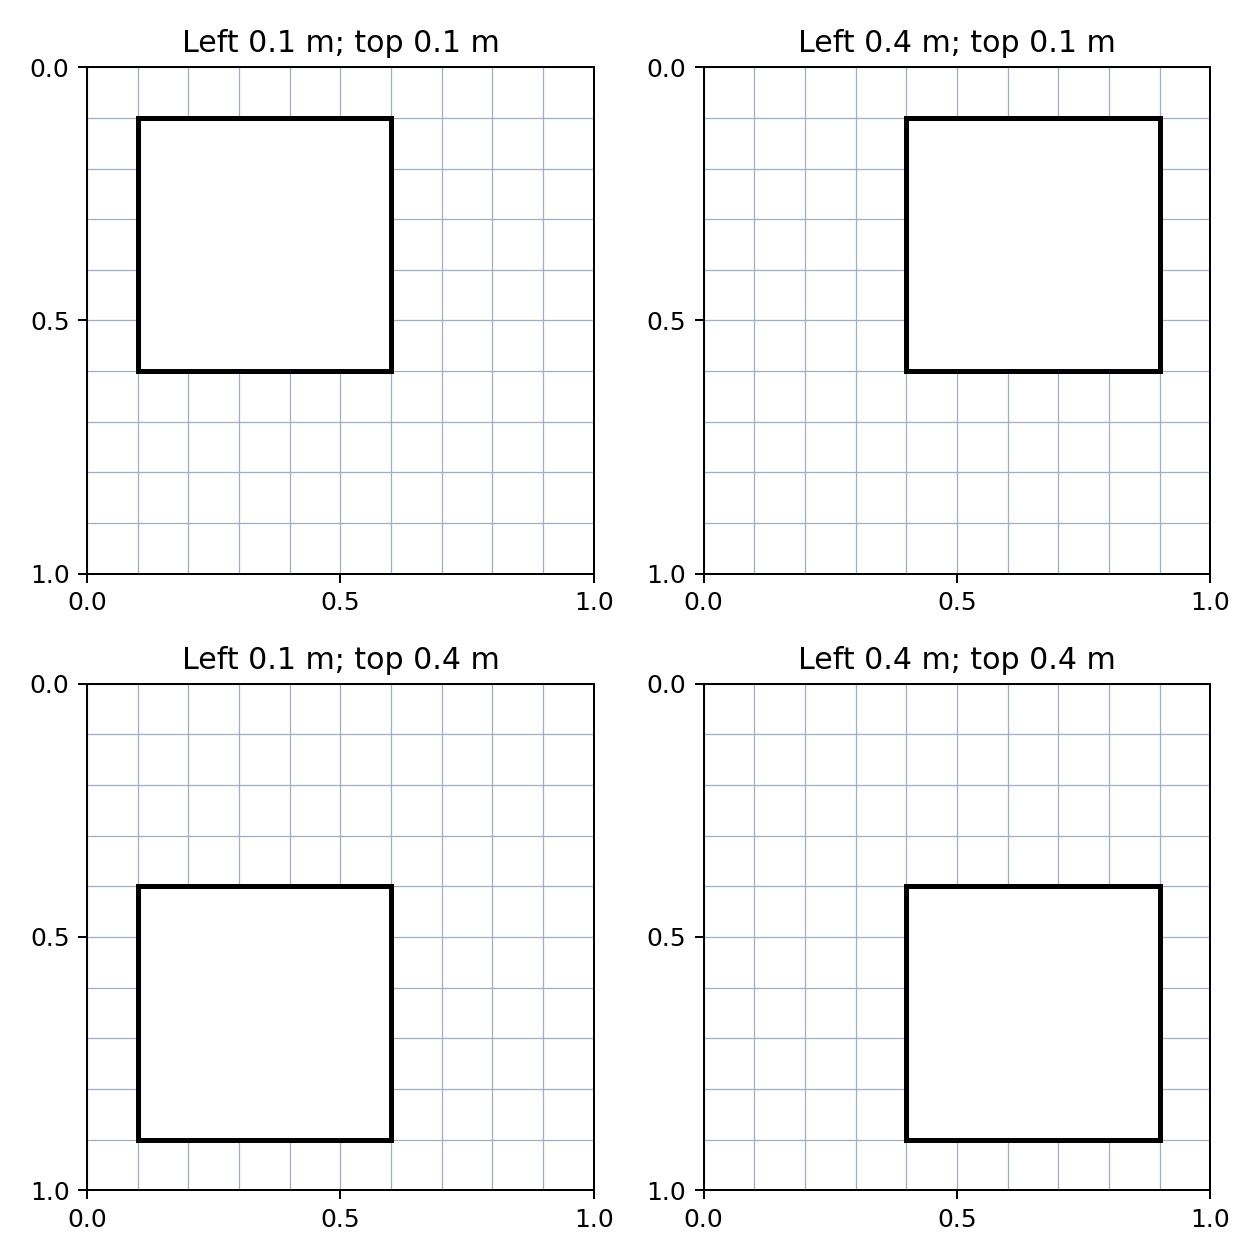
\includegraphics[width=0.94\linewidth,height=0.34\textheight,keepaspectratio]{figures/corner_positions.png}\par

\caption{Reconstructed illustrative corner placements on the permitted grid.}\end{figure}

\begin{figure}[H]\centering

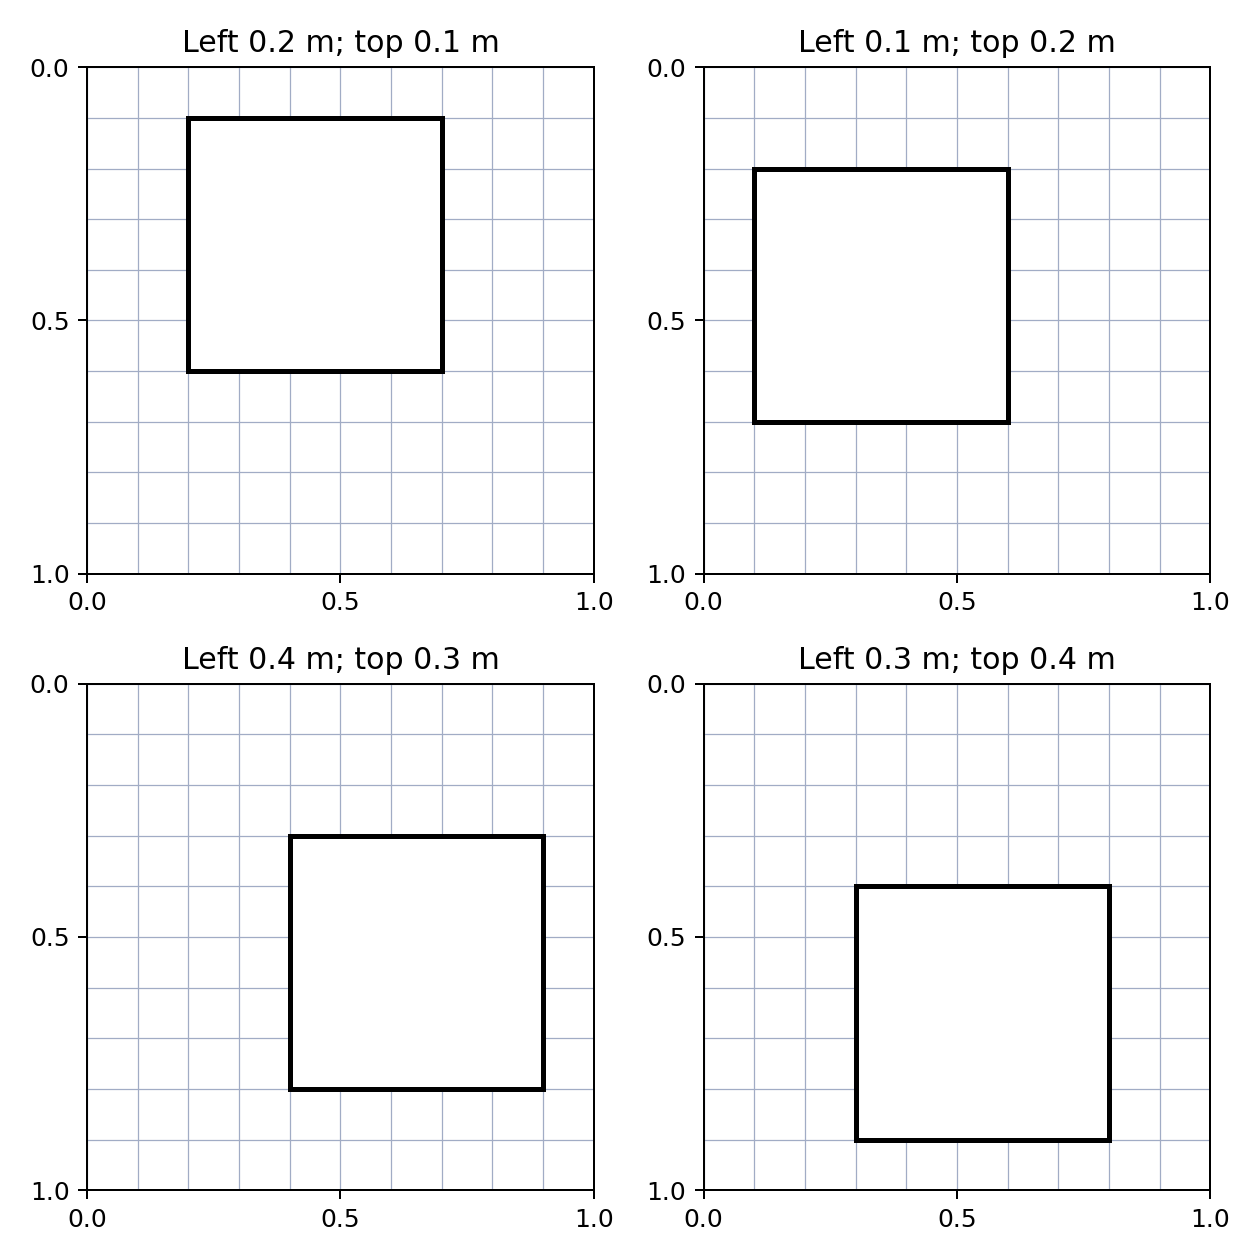
\includegraphics[width=0.94\linewidth,height=0.34\textheight,keepaspectratio]{figures/intermediate_positions.png}\par

\caption{Reconstructed examples of intermediate permitted placements; not a reproduction of Word overlays.}\end{figure}

Each of these preliminary locations can be analyzed before evaluating the full sixteen-position grid.

\section{Problem Description}

The project studies heat transfer through a two-dimensional chimney cross section. The refractory-brick body has a square outside boundary of 1 m by 1 m and contains a square cavity of 0.5 m by 0.5 m. The cavity represents the hot-gas passage, with its wall prescribed at 100 degrees Celsius. The inner square may be positioned asymmetrically, provided the clearance to every corresponding outer wall is at least 10 cm. Moving the cavity within this region permits study of its influence on temperature distribution.

\begin{figure}[H]\centering

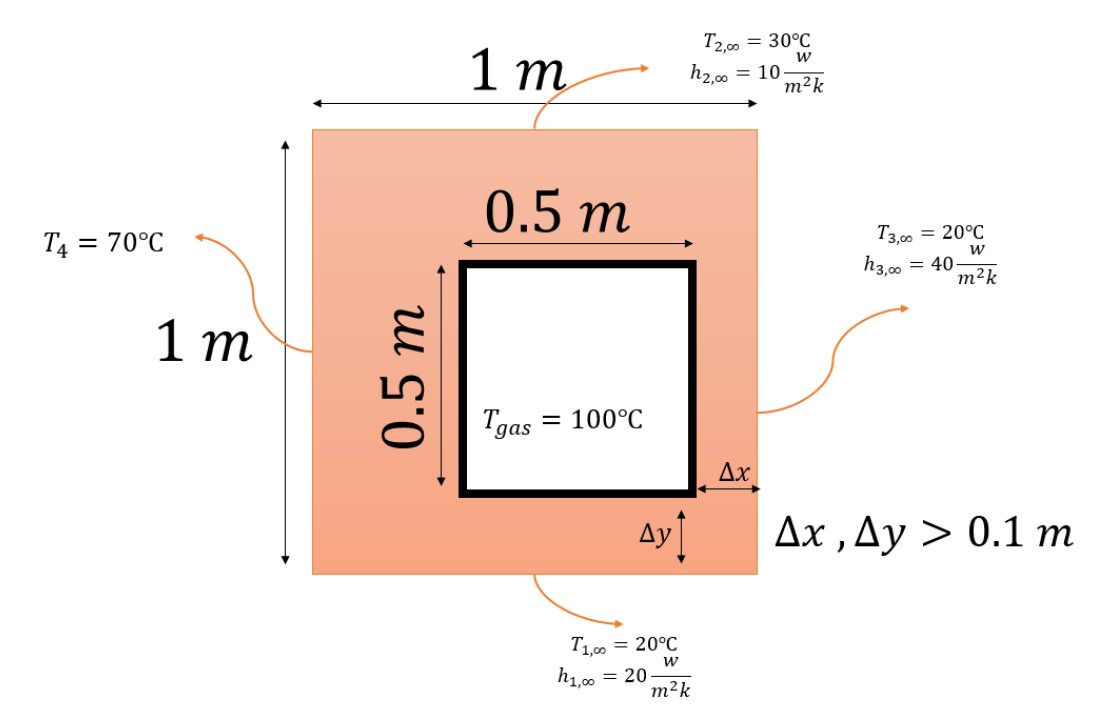
\includegraphics[width=0.94\linewidth,height=0.34\textheight,keepaspectratio]{figures/rId15.png}\par

\caption{Problem geometry and thermal boundary conditions.}\end{figure}

\section{Assumptions}

The inner cavity wall is maintained at $100^\circ$C.

The left outside wall is maintained at $70^\circ$C.

The remaining outside walls, top, right, and bottom, exchange heat by convection with their respective surroundings, using coefficients $h_{i,\infty}$ and ambient temperatures $T_{i,\infty}$.

The refractory brick has constant thermal conductivity and is analyzed at steady state.

Material properties are $\rho=2000\ \mathrm{kg/m^3}$, $k=1\ \mathrm{W/(m\,K)}$, and $C_p=1000\ \mathrm{J/(kg\,K)}$. The code uses bottom, top, and right convection coefficients of 20, 10, and 40 W/(m$^2$ K), respectively, with ambient temperatures of 20, 30, and 20 degrees Celsius.

\section{Hand Formulation}

The upper-left cavity position is used to illustrate the hand calculation.

\begin{figure}[H]\centering


\includegraphics[width=0.94\linewidth,height=0.34\textheight,keepaspectratio]{figures/rId11.png}\par

\caption{Original grid image for the upper-left location; see reconstructed geometry diagrams.}\end{figure}

There are 121 grid nodes. Eleven left-wall nodes have a prescribed temperature of 70 degrees Celsius, and twenty cavity-perimeter nodes have a prescribed temperature of 100 degrees Celsius. Sixteen nodes lie inside the cavity and are not part of the brick. Thus, 74 physical unknown node temperatures remain for each cavity placement.

Nodes are numbered row by row from the upper-left corner: node 1 is at the upper left, node 11 at the upper right, and node 121 at the lower right. For this cavity location, the following nodes share the interior conduction stencil:

19--21, 30--32, 41--43, 52--54, 63--65, 74--76, 79--87, 90--98, and 101--109.

For example, nodes 19 and 109 satisfy

\[T_8+T_{18}+T_{20}+T_{30}-4T_{19}=0.\]

\[T_{98}+T_{108}+T_{110}+T_{120}-4T_{109}=0.\]

The general interior-node equation is

\[T_{m-1,n}+T_{m+1,n}+T_{m,n-1}+T_{m,n+1}-4T_{m,n}=0.\]

The same equation is written for the other listed interior nodes.

Nodes 2--10 share a boundary balance with one convective face and three conductive connections. The grid spacings are $\Delta x=\Delta y=0.1$ m, and a unit axial depth $\Delta z=1$ m is assumed. For node 2,

\[\frac{k\Delta y\Delta z}{2\Delta x}(T_1-T_2)+\frac{k\Delta y\Delta z}{2\Delta x}(T_3-T_2)+\frac{k\Delta x\Delta z}{\Delta y}(T_{13}-T_2)+h_{2,\infty}\Delta x\Delta z(T_{2,\infty}-T_2)=0.\]

The same form applies to bottom nodes 112--120, using $h_{1,\infty}$ and $T_{1,\infty}$ instead. The noncorner right-wall nodes use $h_{3,\infty}$ and $T_{3,\infty}$, with x and y directions exchanged. Because the spacings are equal, the resulting coefficients have the same pattern. The two right corners are treated separately:

\[\begin{aligned}&\frac{k\Delta y\Delta z}{2\Delta x}(T_{10}-T_{11})+\frac{k\Delta x\Delta z}{2\Delta y}(T_{22}-T_{11})\\&\quad+\frac{h_{2,\infty}\Delta x\Delta z}{2}(T_{2,\infty}-T_{11})+\frac{h_{3,\infty}\Delta y\Delta z}{2}(T_{3,\infty}-T_{11})=0.\end{aligned}\]

\[\begin{aligned}&\frac{k\Delta y\Delta z}{2\Delta x}(T_{120}-T_{121})+\frac{k\Delta x\Delta z}{2\Delta y}(T_{110}-T_{121})\\&\quad+\frac{h_{1,\infty}\Delta x\Delta z}{2}(T_{1,\infty}-T_{121})+\frac{h_{3,\infty}\Delta y\Delta z}{2}(T_{3,\infty}-T_{121})=0.\end{aligned}\]

This gives 74 equations for the 74 physical unknown temperatures. Solving the system in MATLAB gives nodal temperatures for subsequent heat-transfer calculations. Changing the cavity location changes the node indices and boundary assignments rather than introducing a different type of governing equation.

\section{MATLAB Solution}

The linear system can be solved efficiently, allowing all sixteen grid-aligned cavity positions to be examined. The coefficient, unknown, and known vectors are arranged as

\[A\mathbf{T}=\mathbf{C}.\]

The code retains a full 121-by-121 matrix A and 121-by-1 vectors T and C, prescribing known grid values to close the system. The formal matrix-inverse expression in the source is

\[\mathbf{T}=A^{-1}\mathbf{C}.\]

\subsection{Original MATLAB code}

\lstinputlisting{../matlab/allstates.m}

A cell array stores the sixteen 11-by-11 temperature arrays.

\begin{figure}[H]\centering

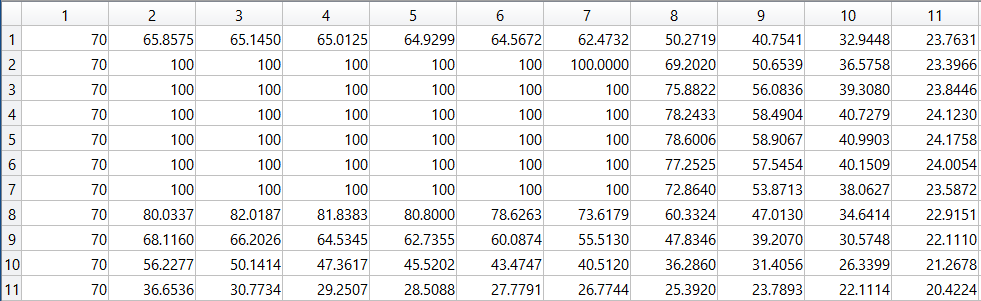
\includegraphics[width=0.94\linewidth,height=0.34\textheight,keepaspectratio]{figures/rId16.png}\par

\caption{Original MATLAB temperature array for State 1.}\end{figure}

\begin{figure}[H]\centering

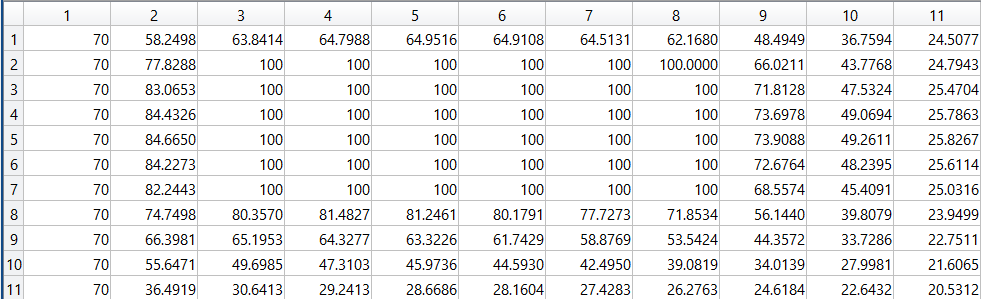
\includegraphics[width=0.94\linewidth,height=0.34\textheight,keepaspectratio]{figures/rId17.png}\par

\caption{Original MATLAB temperature array for State 2.}\end{figure}

\begin{figure}[H]\centering

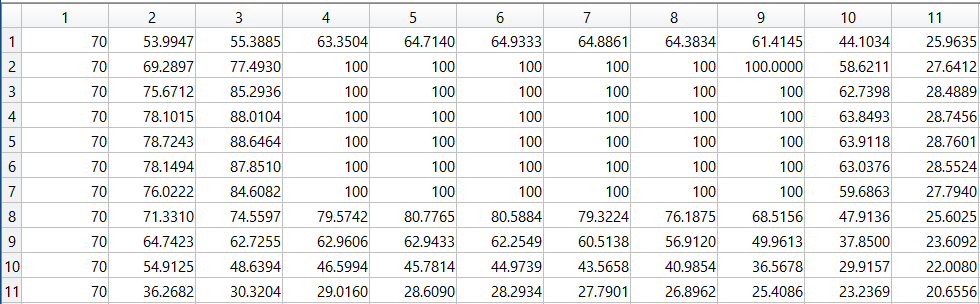
\includegraphics[width=0.94\linewidth,height=0.34\textheight,keepaspectratio]{figures/rId18.png}\par

\caption{Original MATLAB temperature array for State 3.}\end{figure}

\begin{figure}[H]\centering

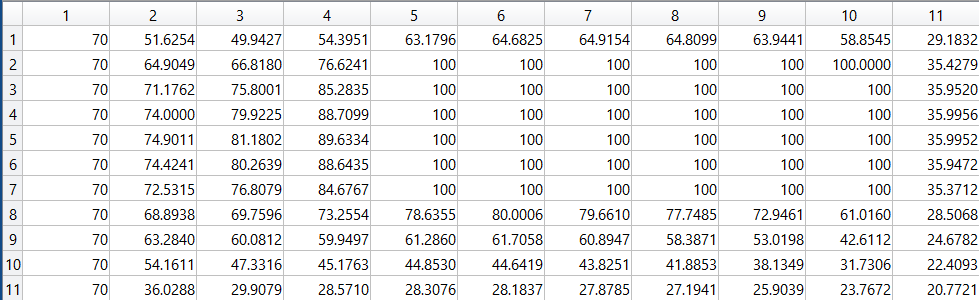
\includegraphics[width=0.94\linewidth,height=0.34\textheight,keepaspectratio]{figures/rId19.png}\par

\caption{Original MATLAB temperature array for State 4.}\end{figure}

\begin{figure}[H]\centering

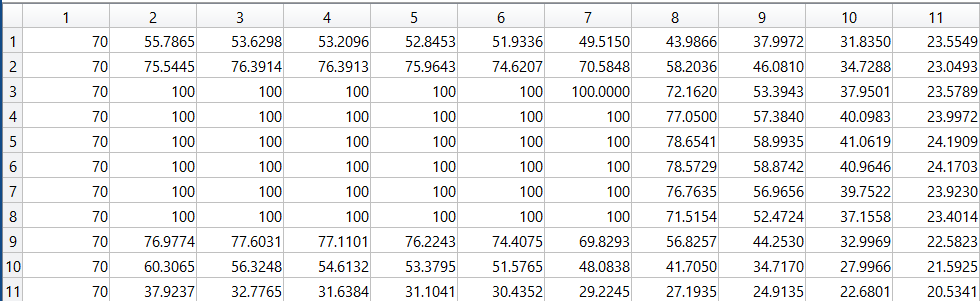
\includegraphics[width=0.94\linewidth,height=0.34\textheight,keepaspectratio]{figures/rId20.png}\par

\caption{Original MATLAB temperature array for State 5.}\end{figure}

\begin{figure}[H]\centering

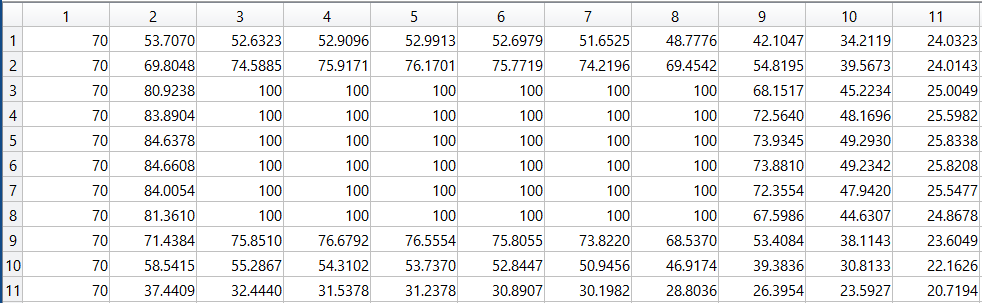
\includegraphics[width=0.94\linewidth,height=0.34\textheight,keepaspectratio]{figures/rId21.png}\par

\caption{Original MATLAB temperature array for State 6.}\end{figure}

\begin{figure}[H]\centering

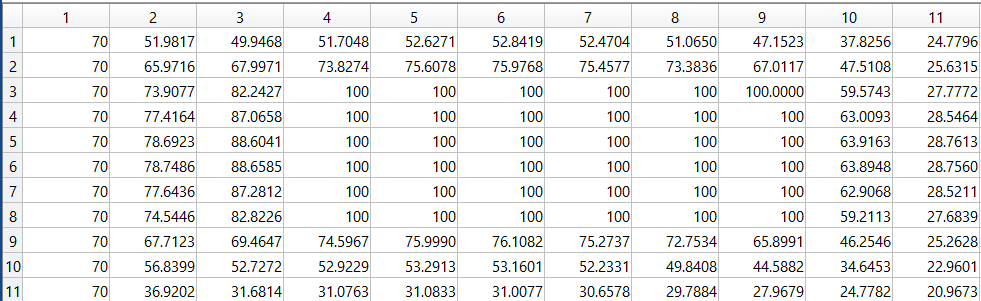
\includegraphics[width=0.94\linewidth,height=0.34\textheight,keepaspectratio]{figures/rId22.png}\par

\caption{Original MATLAB temperature array for State 7.}\end{figure}

\begin{figure}[H]\centering

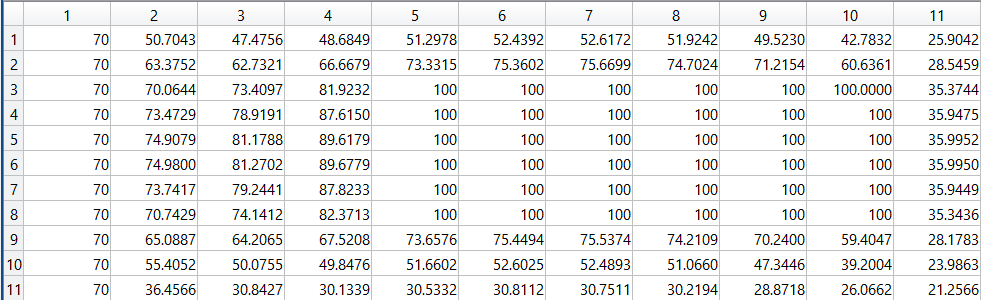
\includegraphics[width=0.94\linewidth,height=0.34\textheight,keepaspectratio]{figures/rId23.png}\par

\caption{Original MATLAB temperature array for State 8.}\end{figure}

\begin{figure}[H]\centering

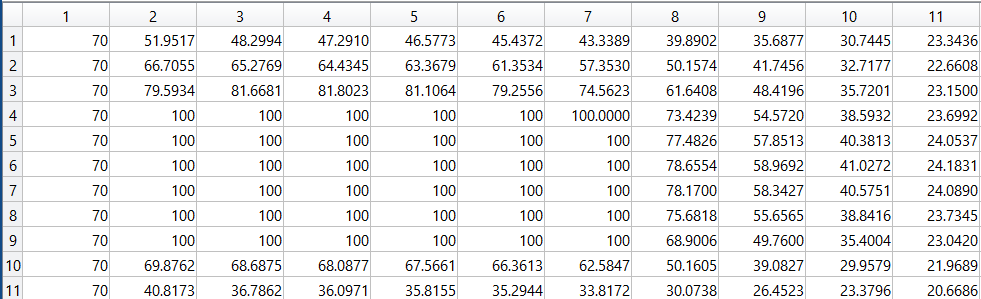
\includegraphics[width=0.94\linewidth,height=0.34\textheight,keepaspectratio]{figures/rId24.png}\par

\caption{Original MATLAB temperature array for State 9.}\end{figure}

\begin{figure}[H]\centering

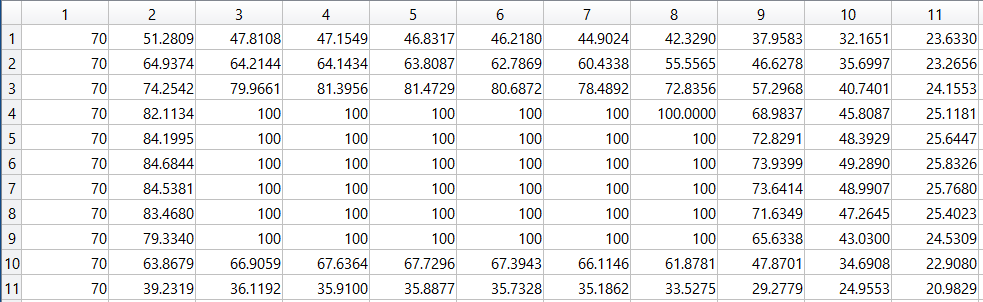
\includegraphics[width=0.94\linewidth,height=0.34\textheight,keepaspectratio]{figures/rId25.png}\par

\caption{Original MATLAB temperature array for State 10.}\end{figure}

\begin{figure}[H]\centering

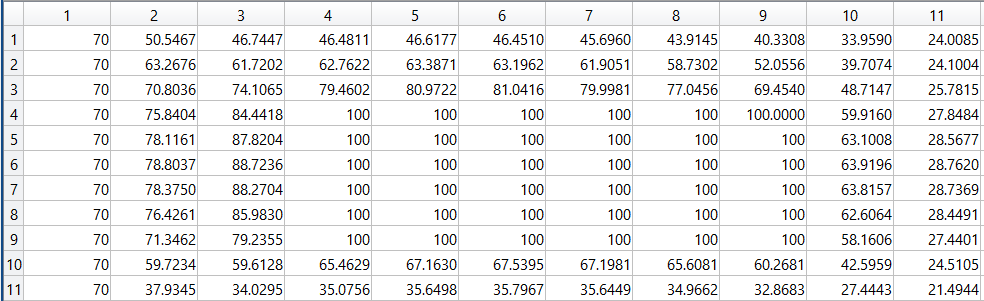
\includegraphics[width=0.94\linewidth,height=0.34\textheight,keepaspectratio]{figures/rId26.png}\par

\caption{Original MATLAB temperature array for State 11.}\end{figure}

\begin{figure}[H]\centering

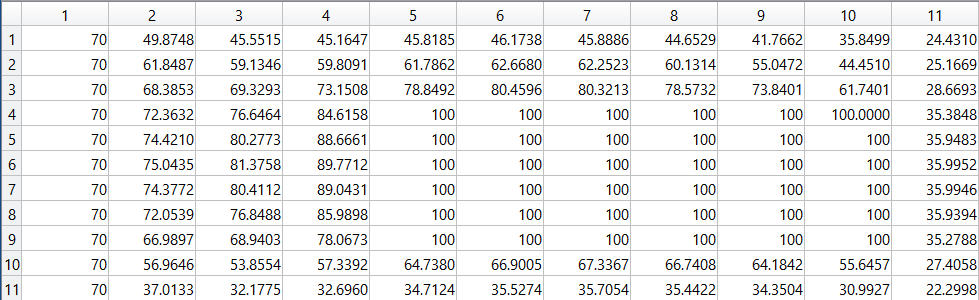
\includegraphics[width=0.94\linewidth,height=0.34\textheight,keepaspectratio]{figures/rId27.png}\par

\caption{Original MATLAB temperature array for State 12.}\end{figure}

\begin{figure}[H]\centering

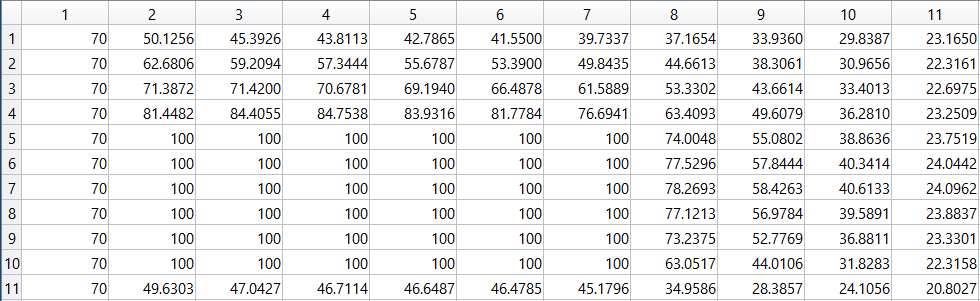
\includegraphics[width=0.94\linewidth,height=0.34\textheight,keepaspectratio]{figures/rId28.png}\par

\caption{Original MATLAB temperature array for State 13.}\end{figure}

\begin{figure}[H]\centering

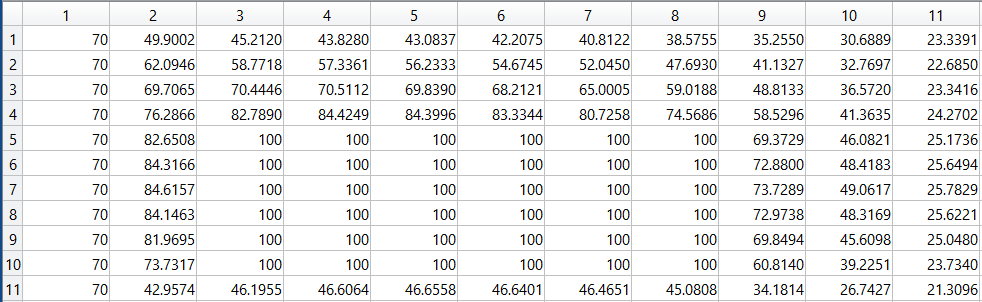
\includegraphics[width=0.94\linewidth,height=0.34\textheight,keepaspectratio]{figures/rId29.png}\par

\caption{Original MATLAB temperature array for State 14.}\end{figure}

\begin{figure}[H]\centering

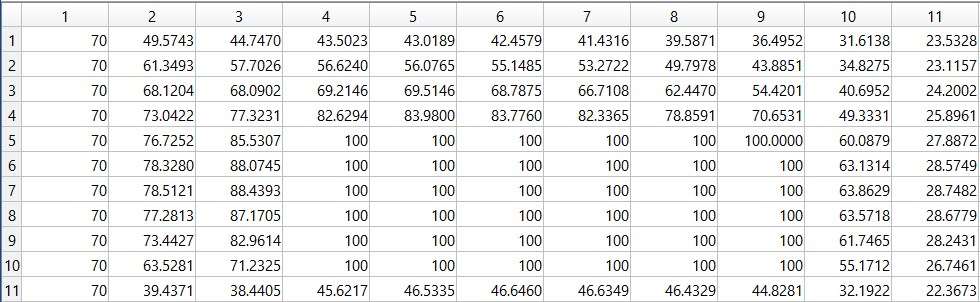
\includegraphics[width=0.94\linewidth,height=0.34\textheight,keepaspectratio]{figures/rId30.png}\par

\caption{Original MATLAB temperature array for State 15.}\end{figure}

\begin{figure}[H]\centering

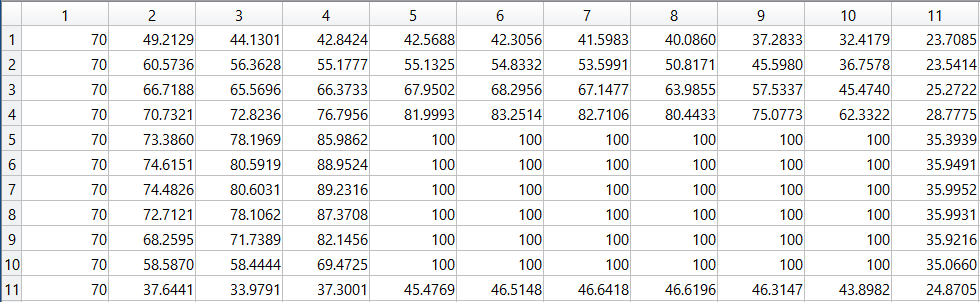
\includegraphics[width=0.94\linewidth,height=0.34\textheight,keepaspectratio]{figures/rId31.png}\par

\caption{Original MATLAB temperature array for State 16.}\end{figure}

The source identifies State 5 as the location with the greatest outward heat-transfer magnitude and reports approximately 18.167 kW. The original calculation uses a signed negative indicator and selects its minimum; the temperature-unit issue is discussed separately in the editorial appendix.

\begin{figure}[H]\centering


\includegraphics[width=0.94\linewidth,height=0.34\textheight,keepaspectratio]{figures/rId11.png}\par

\caption{Original State 5 grid image; its cavity drawing overlay is not embedded in the raster.}\end{figure}

The source places the largest reported heat-transfer magnitude near State 5. It notes that the 10 cm grid is coarse and cannot establish a continuous global optimum. Refining the grid would better resolve the location but increase computation. The source identifies the region near the left wall, between States 1, 5, and 9, as promising, then compares the temperature results with COMSOL.

\begin{figure}[H]\centering

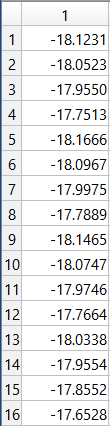
\includegraphics[width=0.94\linewidth,height=0.34\textheight,keepaspectratio]{figures/rId32.png}\par

\caption{Original signed heat-rate indicators for States 1--16.}\end{figure}

\section{COMSOL Model and Comparison}

State 1 is modeled first in COMSOL.

\begin{figure}[H]\centering

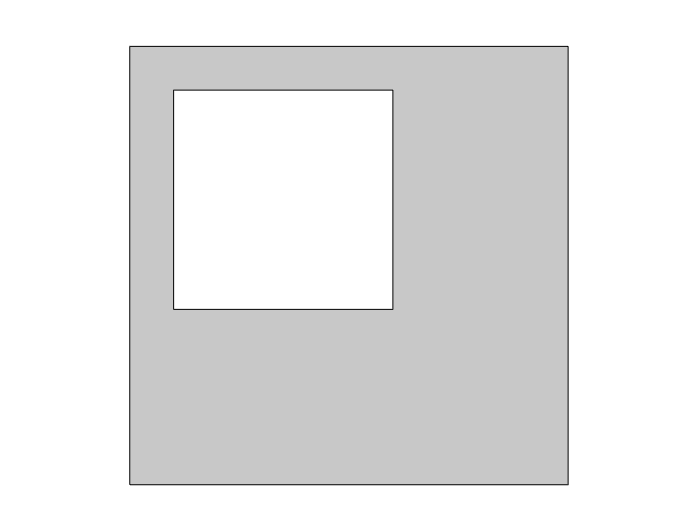
\includegraphics[width=0.94\linewidth,height=0.34\textheight,keepaspectratio]{figures/rId33.png}\par

\caption{State 1 geometry in COMSOL.}\end{figure}

A mesh is generated, and the study is solved.

\begin{figure}[H]\centering

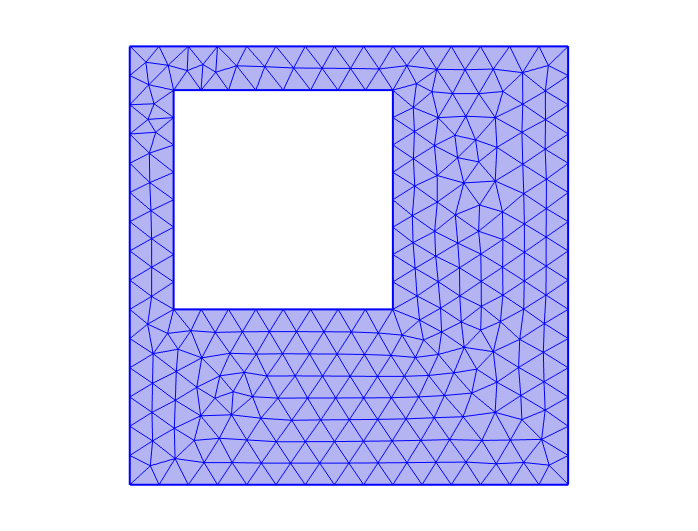
\includegraphics[width=0.94\linewidth,height=0.34\textheight,keepaspectratio]{figures/rId34.png}\par

\caption{State 1 finite-element mesh.}\end{figure}

The temperature distribution and isotherms are displayed.

\begin{figure}[H]\centering

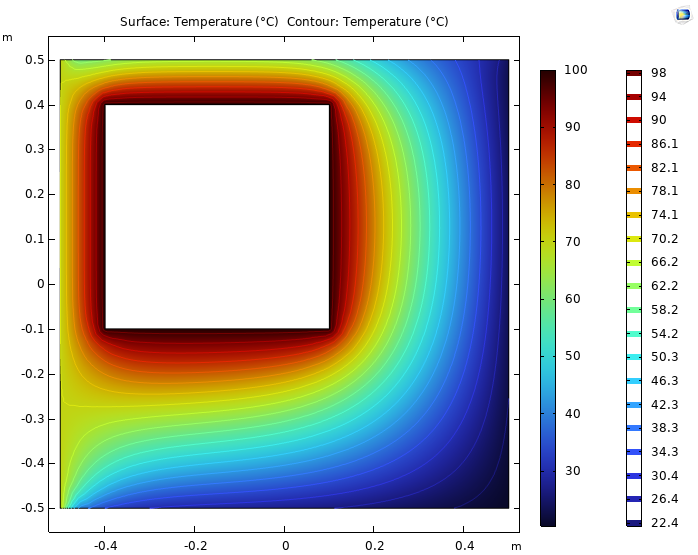
\includegraphics[width=0.94\linewidth,height=0.34\textheight,keepaspectratio]{figures/rId35.png}\par

\caption{State 1 temperature contours and isotherms.}\end{figure}

The source describes the COMSOL temperature range as approximately consistent with the MATLAB State 1 array. Several sample points are compared below. The original table's two group headings appear inconsistent with its data columns; the column labels below follow the row/column node versus coordinate distinction.

\begin{table}[H]\centering\small\caption{Sample point comparison, source values.}\begin{tabular}{rrrrrr}\toprule MATLAB T & Column & Row & COMSOL T & Y & X\\\midrule
23.7631 & 11 & 1 & 23.8929 & 0.5 & 0.5\\20.4224 & 11 & 11 & 20.4105 & -0.5 & 0.5\\22.111 & 11 & 9 & 22.044 & -0.3 & 0.5\\66.2026 & 3 & 9 & 65.3137 & -0.3 & -0.3\\\bottomrule\end{tabular}\end{table}

The source characterizes the sampled temperature differences as being around one percent or less and attributes differences to the coarser MATLAB grid. For heat transfer, it proposes a boundary line integration of normal total heat flux using the COMSOL expression ht.ntflux. The distinction between an integration and summing samples is reviewed in the appendix.

\begin{figure}[H]\centering

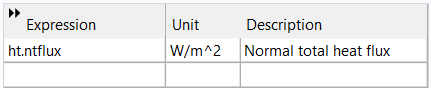
\includegraphics[width=0.94\linewidth,height=0.34\textheight,keepaspectratio]{figures/rId36.png}\par

\caption{COMSOL normal total heat-flux expression.}\end{figure}

The source states that a unit face area does not change its heat-rate value and reports 17292 W for COMSOL State 1 versus 18123 W for MATLAB, describing a discrepancy of about four percent. Its later comparison table reports a different COMSOL State 1 value; both are retained here for traceability.

The calculation is repeated for additional cavity locations.

For the source's State 3 illustration, the temperature and heat rate are obtained in the same way.

\begin{figure}[H]\centering

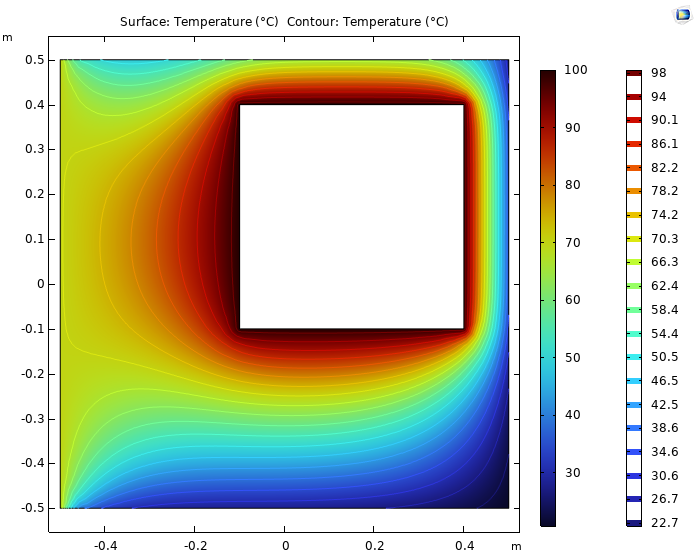
\includegraphics[width=0.94\linewidth,height=0.34\textheight,keepaspectratio]{figures/rId37.png}\par

\caption{Temperature contour labeled State 3 in the source.}\end{figure}

\begin{figure}[H]\centering

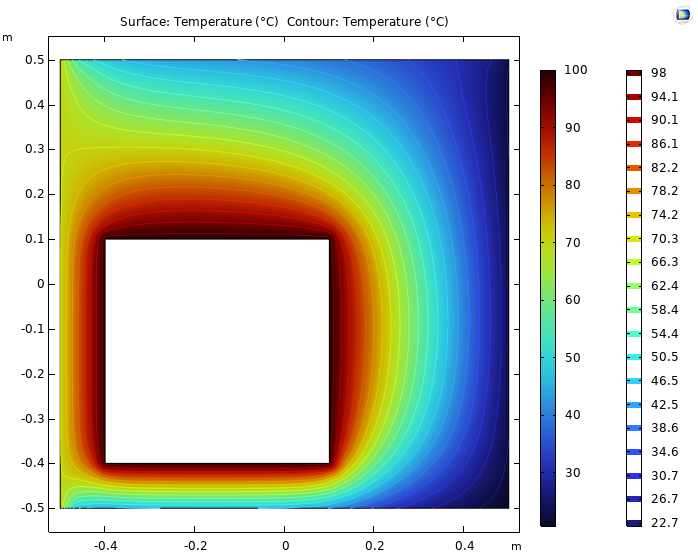
\includegraphics[width=0.94\linewidth,height=0.34\textheight,keepaspectratio]{figures/rId38.png}\par

\caption{State 13 temperature contour.}\end{figure}

The same procedure is shown for State 16.

\begin{figure}[H]\centering

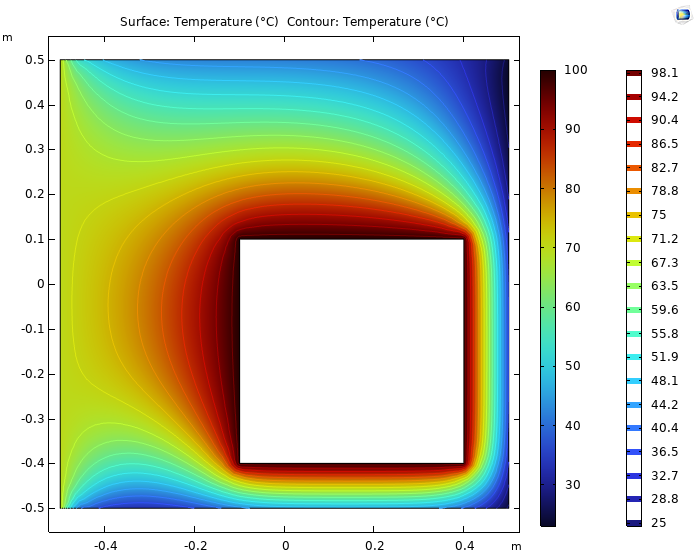
\includegraphics[width=0.94\linewidth,height=0.34\textheight,keepaspectratio]{figures/rId39.png}\par

\caption{State 16 temperature contour.}\end{figure}

The source observes uniform contour color along prescribed-temperature boundaries and isotherms locally parallel to them. The temperature distribution is then shown for State 5, the position selected by the MATLAB indicator.

\begin{figure}[H]\centering

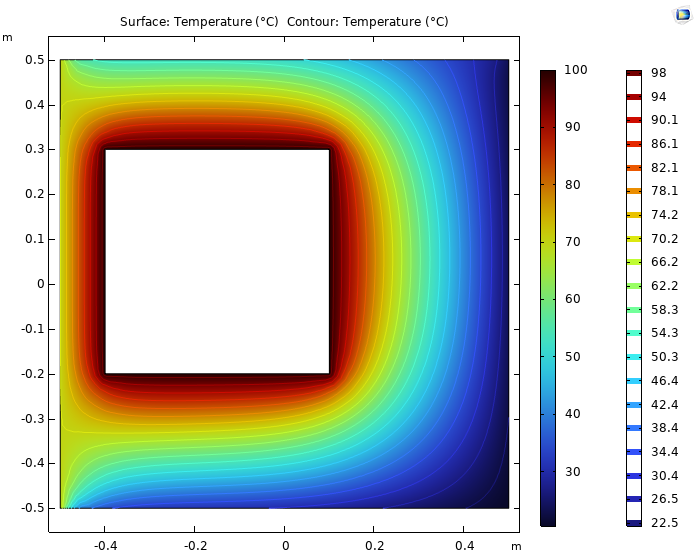
\includegraphics[width=0.94\linewidth,height=0.34\textheight,keepaspectratio]{figures/rId40.png}\par

\caption{State 5 temperature contour.}\end{figure}

State 8 is described as a cavity 20 cm below the top and 10 cm from the right wall.

\begin{figure}[H]\centering

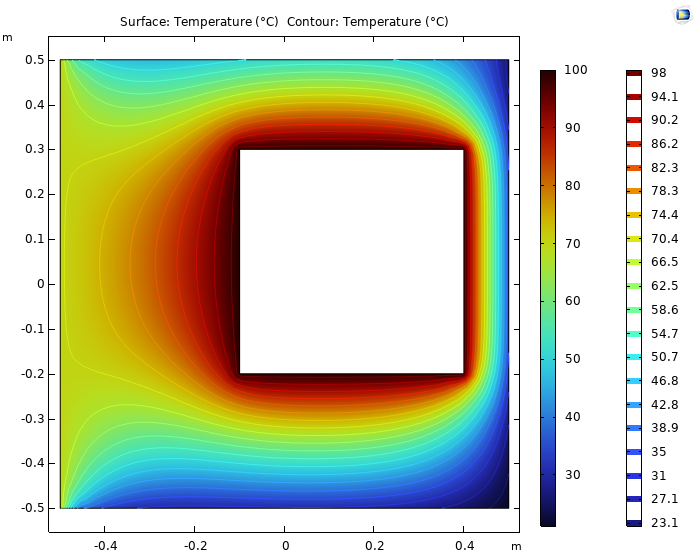
\includegraphics[width=0.94\linewidth,height=0.34\textheight,keepaspectratio]{figures/rId41.png}\par

\caption{State 8 temperature contour.}\end{figure}

State 9 is described as a cavity 20 cm above the bottom and 10 cm from the left wall.

\begin{figure}[H]\centering

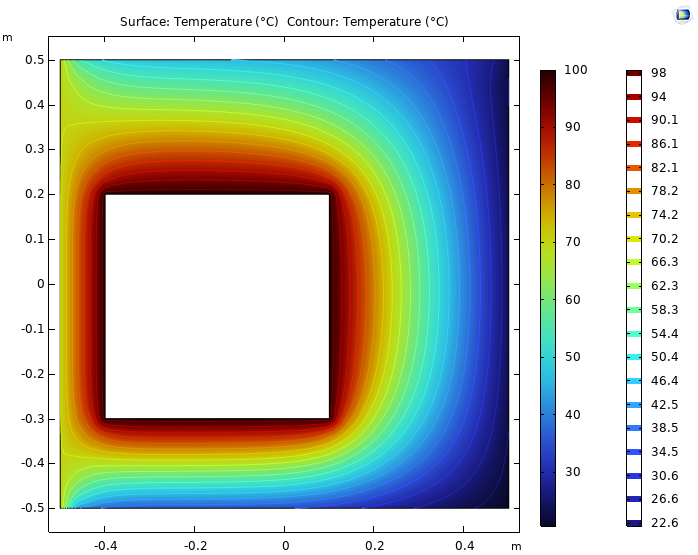
\includegraphics[width=0.94\linewidth,height=0.34\textheight,keepaspectratio]{figures/rId42.png}\par

\caption{State 9 temperature contour.}\end{figure}

State 12 is described as a cavity 20 cm above the bottom and 10 cm from the right wall.

\begin{figure}[H]\centering

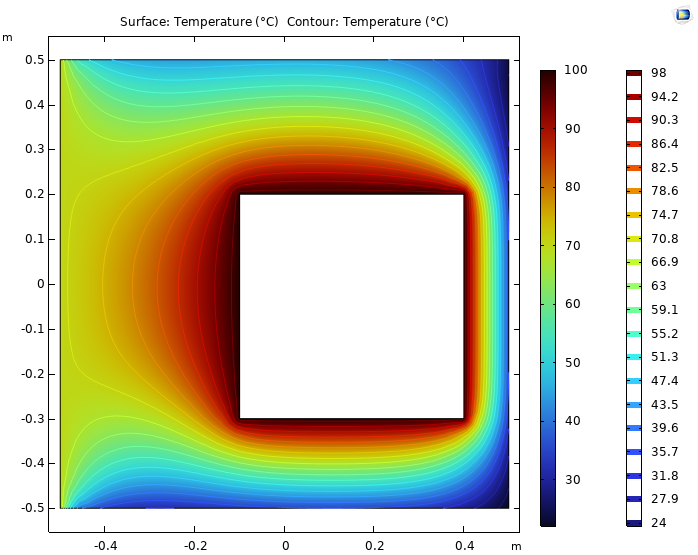
\includegraphics[width=0.94\linewidth,height=0.34\textheight,keepaspectratio]{figures/rId43.png}\par

\caption{State 12 temperature contour.}\end{figure}

The original reported heat-rate comparison is listed below.

\begin{table}[H]\centering\caption{Historical heat-rate comparison, not corrected for the unit inconsistency.}\begin{tabular}{rrr}\toprule COMSOL (kW) & MATLAB (kW) & State\\\midrule-18.123 & -18.1231 & 1\\-17.76 & -17.7513 & 4\\-18.175 & -18.1666 & 5\\-17.845 & -17.7889 & 8\\-18.154 & -18.1465 & 9\\-17.773 & -17.7664 & 12\\-18.034 & -18.0338 & 13\\-17.648 & -17.6528 & 16\\\bottomrule\end{tabular}\end{table}

The source selects State 5 as the best of the compared discrete configurations. These historical heat-rate results require correction and re-evaluation before that selection is used as an engineering design conclusion.

\FloatBarrier\appendix\section{State One COMSOL Point Data}

The following table retains the source appendix's temperature samples for State 1. The coordinate origin is at the center of the chimney cross section. The original text and spreadsheet exports are also included in the repository.

\small\begin{longtable}{rrr}\toprule X (m) & Y (m) & Temperature ($^\circ$C)\\\midrule\endfirsthead\toprule X (m) & Y (m) & Temperature ($^\circ$C)\\\midrule\endhead-0.45326 & -0.45691 & 54.30338\\-0.5 & -0.43333 & 70\\-0.5 & -0.5 & 70\\-0.43333 & -0.5 & 38.09135\\-0.44805 & -0.40007 & 61.42595\\-0.5 & -0.36667 & 70\\-0.36667 & -0.5 & 32.41545\\-0.39682 & -0.44038 & 48.42507\\-0.44942 & -0.33508 & 66.55718\\-0.5 & -0.3 & 70\\-0.39856 & -0.37138 & 59.40153\\-0.33066 & -0.44959 & 41.66711\\-0.3 & -0.5 & 30.3548\\-0.35313 & -0.39907 & 52.14934\\-0.44821 & -0.26869 & 70.39778\\-0.5 & -0.23333 & 70\\-0.39618 & -0.30749 & 66.58001\\-0.44684 & -0.2012 & 74.70343\\-0.5 & -0.16667 & 70\\-0.2665 & -0.4496 & 39.42791\\-0.23333 & -0.5 & 29.38578\\-0.33834 & -0.34289 & 60.12952\\-0.29581 & -0.39413 & 50.3269\\-0.34727 & -0.2777 & 69.46756\\-0.30605 & -0.30281 & 65.31366\\-0.39403 & -0.24168 & 73.62712\\-0.38987 & -0.19097 & 80.11538\\-0.45929 & -0.13367 & 77.88543\\-0.5 & -0.1 & 70\\-0.45034 & -0.07054 & 83.73102\\-0.5 & -0.03333 & 70\\-0.45008 & -0.00385 & 84.84022\\-0.414 & -0.15482 & 83.02815\\-0.4 & -0.0375 & 100\\-0.5 & 0.033333 & 70\\-0.45031 & 0.061197 & 84.88921\\-0.4 & 0.025 & 100\\-0.19994 & -0.45067 & 37.94308\\-0.16667 & -0.5 & 28.80724\\-0.23305 & -0.39785 & 47.93508\\-0.26811 & -0.34058 & 58.51765\\-0.2643 & -0.28791 & 67.07892\\-0.29464 & -0.25176 & 73.14723\\-0.3358 & -0.21059 & 79.29199\\-0.36061 & -0.14864 & 89.02244\\-0.4 & -0.1 & 100\\-0.5 & 0.1 & 70\\-0.45179 & 0.125203 & 84.46072\\-0.4 & 0.0875 & 100\\-0.13343 & -0.45094 & 36.97098\\-0.1 & -0.5 & 28.33797\\-0.16589 & -0.40194 & 45.92005\\-0.20096 & -0.34832 & 55.83952\\-0.22004 & -0.29932 & 64.54915\\-0.23899 & -0.24368 & 74.23179\\-0.27158 & -0.20027 & 81.72972\\-0.30533 & -0.15264 & 89.88742\\-0.3375 & -0.1 & 100\\-0.06674 & -0.45093 & 36.07558\\-0.03333 & -0.5 & 27.84294\\-2.33E-04 & -0.4507 & 35.06718\\0.033333 & -0.5 & 27.24973\\-0.5 & 0.166667 & 70\\-0.45453 & 0.18909 & 83.63367\\-0.4 & 0.15 & 100\\-0.09968 & -0.40192 & 44.75782\\-0.13068 & -0.3531 & 53.68614\\-0.16208 & -0.30251 & 63.05948\\-0.18711 & -0.25211 & 72.26692\\-0.21145 & -0.20211 & 81.33266\\-0.24322 & -0.15121 & 90.55183\\-0.275 & -0.1 & 100\\-0.0331 & -0.40167 & 43.45626\\0.032917 & -0.40094 & 41.88311\\0.066094 & -0.45027 & 33.83816\\0.1 & -0.5 & 26.52489\\-0.5 & 0.233333 & 70\\-0.45541 & 0.256021 & 83.32658\\-0.4 & 0.2125 & 100\\-0.06457 & -0.35218 & 52.40397\\-0.09449 & -0.30232 & 61.74365\\-0.12298 & -0.25186 & 71.34861\\-0.15168 & -0.2013 & 80.99589\\-0.18159 & -0.15082 & 90.53026\\-0.2125 & -0.1 & 100\\6.71E-04 & -0.3517 & 50.62794\\0.065401 & -0.35107 & 48.27281\\0.098387 & -0.40014 & 39.87681\\0.132197 & -0.44973 & 32.33581\\0.166667 & -0.5 & 25.66788\\-0.5 & 0.3 & 70\\-0.4409 & 0.303871 & 87.5043\\-0.4 & 0.275 & 100\\-0.45853 & 0.333287 & 81.89348\\-0.03046 & -0.30214 & 60.01595\\-0.06039 & -0.25212 & 69.89882\\-0.08989 & -0.20164 & 80.05144\\-0.11968 & -0.15091 & 90.15729\\-0.15 & -0.1 & 100\\0.033333 & -0.30202 & 57.54309\\0.096682 & -0.3016 & 54.18735\\0.129842 & -0.34988 & 45.31779\\0.163682 & -0.39888 & 37.47207\\0.198415 & -0.44903 & 30.57823\\0.233333 & -0.5 & 24.70351\\-0.5 & 0.366667 & 70\\-0.4 & 0.3375 & 100\\-0.44469 & 0.368971 & 84.73389\\0.002621 & -0.25245 & 67.66213\\-0.02734 & -0.20204 & 78.47058\\-0.05732 & -0.1511 & 89.45052\\-0.0875 & -0.1 & 100\\0.064943 & -0.25309 & 64.2135\\0.126323 & -0.25277 & 59.57194\\0.158764 & -0.29973 & 50.18287\\0.266807 & -0.44851 & 28.52671\\0.3 & -0.5 & 23.66781\\0.194256 & -0.34724 & 41.91427\\0.229496 & -0.39715 & 34.70206\\0.335751 & -0.45222 & 26.0605\\0.366667 & -0.5 & 22.59398\\-0.45698 & 0.412359 & 77.51995\\-0.5 & 0.433333 & 70\\-0.46342 & 0.463647 & 69.18242\\-0.5 & 0.5 & 70\\-0.4 & 0.4 & 100\\0.035165 & -0.20298 & 75.61103\\0.005358 & -0.15158 & 88.04667\\-0.025 & -0.1 & 100\\0.095619 & -0.20506 & 70.63709\\0.151403 & -0.20979 & 63.74577\\0.181723 & -0.25085 & 54.61513\\0.217441 & -0.2966 & 45.89947\\0.303091 & -0.39898 & 30.99512\\0.26019 & -0.34498 & 37.8933\\0.368052 & -0.3981 & 27.83669\\0.39829 & -0.44934 & 24.18694\\0.433333 & -0.5 & 21.50447\\0.456569 & -0.45544 & 22.12504\\0.5 & -0.5 & 20.41047\\-0.41266 & 0.45677 & 74.28596\\-0.43333 & 0.5 & 60.59833\\-0.36908 & 0.444671 & 81.92363\\-0.3375 & 0.4 & 100\\0.066778 & -0.15396 & 84.39056\\0.0375 & -0.1 & 100\\0.12111 & -0.15882 & 76.79338\\0.170085 & -0.17002 & 67.28704\\0.203923 & -0.20292 & 58.12776\\0.239062 & -0.24481 & 49.33625\\0.28002 & -0.29106 & 41.07527\\0.33334 & -0.33503 & 33.59523\\0.39434 & -0.35151 & 28.53306\\0.439389 & -0.39662 & 24.31465\\0.5 & -0.43333 & 20.958\\-0.36667 & 0.5 & 62.98911\\-0.33321 & 0.458587 & 78.28239\\-0.30396 & 0.440974 & 85.11392\\-0.275 & 0.4 & 100\\0.1 & -0.1 & 100\\0.160956 & -0.12447 & 75.63555\\0.211211 & -0.15147 & 63.0769\\0.262801 & -0.18673 & 52.01083\\0.291415 & -0.23644 & 44.4078\\0.337329 & -0.2662 & 37.60572\\0.391867 & -0.29664 & 31.09191\\0.4475 & -0.32986 & 25.59981\\0.5 & -0.36667 & 21.5046\\-0.2125 & 0.4 & 100\\-0.25617 & 0.455559 & 80.3042\\-0.3 & 0.5 & 64.41057\\0.155241 & -0.06943 & 83.3806\\0.1 & -0.0375 & 100\\0.208856 & -0.09745 & 68.95458\\0.25613 & -0.12875 & 57.87397\\0.300476 & -0.14742 & 49.73185\\0.329145 & -0.19654 & 42.79613\\0.386954 & -0.23255 & 34.33552\\0.444823 & -0.26513 & 27.45725\\0.5 & -0.3 & 22.04405\\-0.15 & 0.4 & 100\\-0.19232 & 0.453543 & 81.17681\\-0.23333 & 0.5 & 64.83684\\0.15083 & -0.00635 & 87.52672\\0.1 & 0.025 & 100\\0.203501 & -0.0369 & 74.2827\\0.252742 & -0.06937 & 62.60305\\0.301886 & -0.09311 & 52.73471\\0.345353 & -0.12794 & 44.33209\\0.389363 & -0.16857 & 36.65783\\0.44337 & -0.19806 & 29.25168\\0.5 & -0.23333 & 22.56279\\-0.0875 & 0.4 & 100\\-0.12632 & 0.450596 & 82.20856\\-0.16667 & 0.5 & 64.9288\\0.146075 & 0.052109 & 89.59665\\0.1 & 0.0875 & 100\\0.197755 & 0.021231 & 77.6953\\0.251992 & -0.00526 & 65.73829\\0.301507 & -0.03612 & 55.3923\\0.351038 & -0.06769 & 45.93726\\0.398643 & -0.09923 & 37.71057\\0.445485 & -0.13233 & 30.41994\\0.5 & -0.16667 & 23.03935\\-0.06145 & 0.450034 & 82.23831\\-0.025 & 0.4 & 100\\-0.1 & 0.5 & 64.86984\\0.144407 & 0.113655 & 90.29912\\0.1 & 0.15 & 100\\0.19543 & 0.077719 & 79.1651\\0.24807 & 0.051126 & 67.98889\\0.300686 & 0.026093 & 57.40212\\0.350479 & -0.00377 & 47.89389\\0.399705 & -0.03535 & 39.12563\\0.449312 & -0.06743 & 31.00046\\0.5 & -0.1 & 23.4481\\0.003439 & 0.449606 & 81.71983\\0.0375 & 0.4 & 100\\-0.03333 & 0.5 & 64.53596\\0.149949 & 0.181451 & 88.98271\\0.1 & 0.2125 & 100\\0.146925 & 0.24367 & 89.0492\\0.1 & 0.275 & 100\\0.201369 & 0.144711 & 78.17736\\0.242502 & 0.115587 & 69.76943\\0.295656 & 0.078188 & 59.19026\\0.351036 & 0.059394 & 48.89833\\0.39998 & 0.030328 & 40.16084\\0.449777 & -0.00125 & 31.73729\\0.5 & -0.03333 & 23.76611\\0.06866 & 0.448366 & 79.40389\\0.1 & 0.4 & 100\\0.033333 & 0.5 & 63.27869\\0.201157 & 0.205266 & 77.7139\\0.14657 & 0.360377 & 84.4937\\0.1 & 0.3375 & 100\\0.149262 & 0.305651 & 87.00013\\0.194912 & 0.27343 & 77.41625\\0.261882 & 0.188303 & 65.59357\\0.29795 & 0.137998 & 59.02279\\0.350087 & 0.122346 & 49.46972\\0.400035 & 0.094907 & 40.67906\\0.449668 & 0.064963 & 32.23451\\0.5 & 0.033333 & 23.97876\\0.153904 & 0.414787 & 74.16288\\0.189246 & 0.39648 & 69.12939\\0.132002 & 0.455912 & 68.48366\\0.1 & 0.5 & 59.51144\\0.247813 & 0.246075 & 67.20583\\0.203397 & 0.337277 & 72.13164\\0.241427 & 0.296993 & 66.55806\\0.29599 & 0.23638 & 58.17651\\0.333448 & 0.192712 & 52.09383\\0.398619 & 0.163928 & 40.90923\\0.450043 & 0.129907 & 32.32158\\0.5 & 0.1 & 24.08083\\0.236373 & 0.39216 & 60.34488\\0.200416 & 0.44758 & 58.85298\\0.166667 & 0.5 & 52.75198\\0.288795 & 0.286515 & 57.93597\\0.266441 & 0.340564 & 59.24434\\0.337451 & 0.269532 & 49.87056\\0.396416 & 0.230946 & 40.67979\\0.450249 & 0.196883 & 32.10738\\0.5 & 0.166667 & 24.0715\\0.296201 & 0.392049 & 50.57699\\0.264617 & 0.446571 & 49.82981\\0.233333 & 0.5 & 45.98845\\0.333745 & 0.337493 & 48.01086\\0.394479 & 0.304045 & 39.61761\\0.447434 & 0.265465 & 32.01017\\0.5 & 0.233333 & 23.94989\\0.351061 & 0.396986 & 42.5225\\0.329097 & 0.448085 & 42.03526\\0.3 & 0.5 & 40.27347\\0.396411 & 0.368087 & 37.54402\\0.448244 & 0.332787 & 31.00315\\0.5 & 0.3 & 23.72017\\0.395905 & 0.439885 & 35.19481\\0.366667 & 0.5 & 35.29074\\0.447813 & 0.398161 & 30.01233\\0.5 & 0.366667 & 23.41358\\0.454748 & 0.456318 & 28.50307\\0.433333 & 0.5 & 30.38475\\0.5 & 0.433333 & 23.17201\\0.5 & 0.5 & 23.89287\\\bottomrule\end{longtable}\normalsize

\section{Editorial Review}
The source uses TC/Vis in Celsius for most convective surface terms but retains ambient T1, T2, and T3 in kelvin. Temperature differences must use a consistent scale. Some corner terms use T4 in kelvin while others use Vis in Celsius. The resulting sum therefore cannot be treated as a physical heat rate. This issue affects both supplied MATLAB scripts and the reported State 5 selection. Their numerical logic is preserved rather than silently repaired.

The outer heat-transfer sum also includes convection on the top, bottom, and right walls, but does not include conductive exchange through the prescribed-temperature left wall. Thus, even after correcting units, it should not automatically be called total heat transfer through the entire outer boundary. An independent energy balance and a declared objective are needed.

The code variable maxq is assigned min(Qall), selecting the most negative signed value. Largest signed value, largest outward heat rate, and largest magnitude are different objectives. The sign convention must be established before choosing an optimum. A coarse sixteen-point placement search is not proof of a continuous global optimum; no mesh-convergence study is supplied.

The report's COMSOL State 1 prose quotes 17292 W, while its final table quotes -18.123 kW. The prose also discusses State 3, whereas the final table lists State 4. These inconsistencies must be reconciled with the saved models and exact boundary selections. Small differences in selected temperatures do not validate an inconsistent heat-rate calculation.

COMSOL ht.ntflux is a normal heat-flux quantity. To obtain heat rate for a two-dimensional section, integrate along the specified boundary with the intended out-of-plane depth and sign convention. Summing point samples is not generally the same as boundary integration. Inspect the saved evaluation method before accepting the historical comparison values.

The code fills the whole cavity block with the prescribed gas temperature, including interior placeholder nodes, but those nodes are not physical brick temperatures. Distinguish placeholders from material-domain results. Density and heat capacity are listed material properties, but they do not enter a steady constant-conductivity temperature equation without transient storage.

The native archive includes eleven COMSOL MPH models, two MATLAB Live Scripts, and text/spreadsheet point exports. It does not include a native model for every one of the sixteen placements. The exported point table and the source appendix may use different precision or sampling; both are preserved independently. The two extracted M files are text versions of the supplied code, not corrected implementations. Neither MATLAB nor COMSOL was executed during conversion. No solver validation, physical experiment, or manufacturing design approval is claimed.
\end{document}